\subsection{Initial Conditions}
\label{subsec:init}

As mention in section \ref{sec:structure}, the code starts off by reading a set of initial conditions.
These are organized as a set of $6 \times N$ phase-space arrays -- one per {\small MPI} process -- where $N$ is the number of particles in the
local volume. Although many applications are typically based on initial conditions that follow Gaussian statistics,
we have developed a non-Gaussian initial conditions generator that we briefly describe in this section. 


The original code that provides Gaussian initial conditions for {\small CUBEP3M} 
is extended to include non-Gaussian features of the `local' form,
$\Phi({\bf x})=\phi({\bf x})+f_{\rm NL} \phi({\bf x})^2 + g_{\rm NL} 
\phi({\bf x})^3$, where $\phi({\bf x})$ is the Gaussian contribution
to the Bardeen potential $\Phi({\bf x})$ (see \cite{2004PhR...402..103B} for a review). 
We adopted the CMB convention,
in which $\Phi$ is calculated immediately after the matter-
radiation equality (and not at redshift $z=0$ as in the large scale
structure convention). For consistency, $\phi({\bf x})$ is normalized
to the amplitude of scalar perturbations inferred by CMB measurements
($A_s\approx 2.2 \times 10^{-9}$). The local transformation is performed 
before the inclusion of the matter transfer function, and the initial 
particle positions and velocities are finally computed from $\Phi({\bf x})$ 
according to the Zel'dovich approximation, as in the original Gaussian initial condition generator.

This code was tested by comparing simulations and theoretical predictions
for the effect of local primordial non-Gaussianity on the halo mass 
function and matter power spectrum (Desjacques, Seljak \& Iliev 2009). 
It has also been used to quantify the impact of local non-Gaussian initial
conditions on the halo power spectrum \citep{2009MNRAS.396...85D,
2010PhRvD..81b3006D} and bispectrum \citep{2010MNRAS.406.1014S},
 as well as the matter bispectrum \citep{2011arXiv1111.6966S}.
Fig. \ref{fig:init} shows the late time power spectrum of two realizations that started off the same initial power spectrum, 
but one of which had non-Gaussian initial conditions.
We see that the difference between the two power spectra is at the sub-per cent level, but that the non-Gaussian realization
agrees much better with one loop perturbation theory \citep{XXX}.

\begin{figure}%[ht]
  \begin{center}
    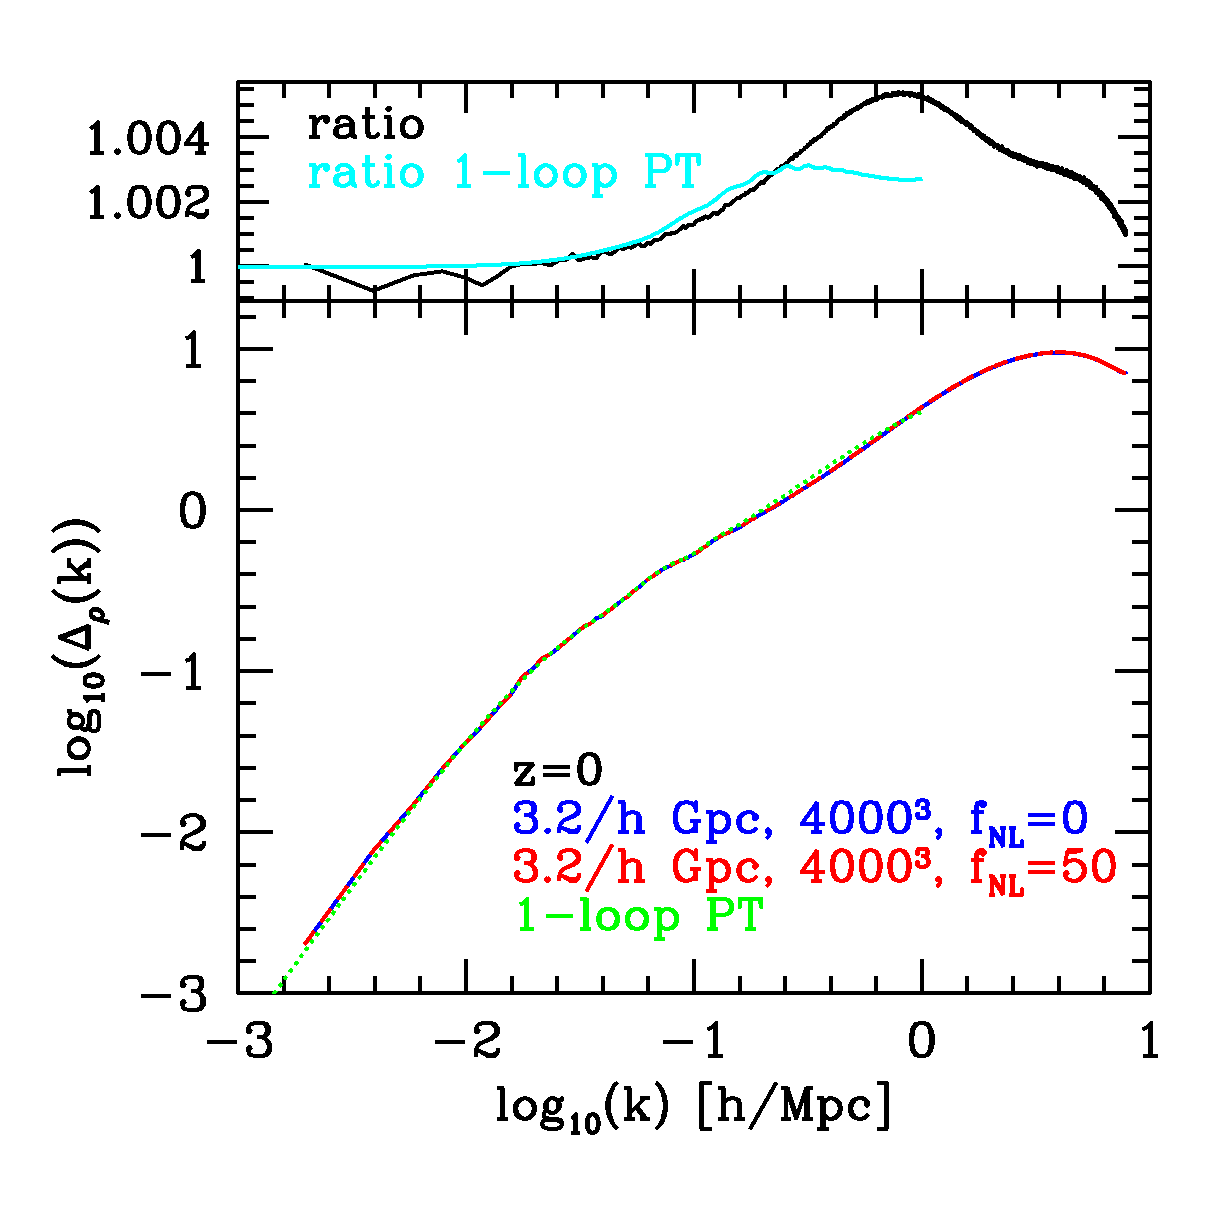
\includegraphics[width=3.2in]{graphs/dm_power_z0_fNL0_50_w_1loop_PT.eps}
  \caption{ Dark matter power spectrum, measured at $z=0$ in a volume $3.2 h^{-1}\mbox{Gpc}$ per side,
  from $4000^3$ particles. The two curves represent two realizations of the same initial power spectrum, one of which used Gaussian statistics (blue) and the other the non-Gaussian initial condition generator. The to curves differ at the sub-per cent level, as seen in the top panel.   
    \label{fig:init}}
\end{center}
\end{figure}

